\documentclass[answers]{exam}
 
\usepackage{graphicx}
\usepackage{float}
\usepackage{amsmath}
\usepackage{amsthm}
\usepackage{subcaption}
\usepackage{framed}
\usepackage{algpseudocode}
\usepackage{tikz}

\newtheorem{lemma}{Lemma}
\newtheorem{claim}{Claim}
\newcommand{\nl}{\vspace{0.2cm}\\}
\newcommand{\nln}{\vspace{0.2cm}}

 
% First we setup the header and footer
\pagestyle{headandfoot}
\runningheadrule
\runningfootrule
\header{COL351: Analysis and Design of Algorithms (CSE, IITD, Semester-I-2020-21)}{}{Homework-2}
\footer{}{\thepage  \, of \numpages}{}
 
% We want the points for each question displayed on the left
%\pointname{points}
%\pointsinmargin
 
% Automatically total the points - make sure to compile TWICE
\addpoints
 
\begin{document}


\begin{center} 
\fbox{\parbox{5.5in}{
\vspace{-0.1in}
\begin{itemize}
\item \small{The instructions are the same as in Homework-0, 1.}
\end{itemize}
\vspace{-0.1in}
}}
\end{center}

\vspace{0.1in}


\vspace{0.1in}
% Some general text together with number of questions and total points possible
There are \numquestions\, questions for a total of \numpoints\, points.
\vspace{0.1in}
\hrule
 \vspace{0.2in}
\begin{questions}
 
% First question, worth 3 points
\question[12] Given a strongly connected directed graph, $G = (V, E)$ with positive edge weights along with a particular node $v \in V$. 
You wish to pre-process the graph so that queries of the form ``what is the length of the shortest path from $s$ to $t$ that goes through $v$" can be answered in constant time for any pair of distinct vertices $s$ and $t$. The pre-processing should take the same asymptotic run-time as Dijkstra's algorithm. Analyse the runtime and provide a proof of correctness.

\begin{solution}\nl
\textbf{Algorithm:}
\begin{algorithmic}[1]
    \Function{Problem1PreProcessing}{$G, v$}
        \State let $G^{R} \gets$ \Call{Reverse}{$G$}
        \State let $D_{1} \gets$ \Call{Dijkstra}{$G^{R}, v$}
        \State let $D_{2} \gets$ \Call{Dijkstra}{$G, v$}
        \State \Return $(D_1, D_2)$
    \EndFunction
    \Function{Problem1Queries}{$G, v,$ stream of queries}
        \State let $(D_1, D_2) \gets$ \Call{Problem1PreProcessing}{$G, v$}
        \While{there are queries to process}
            \State let $s, t$ = current query
            \State output $D_1[s] + D_2[t]$
            \State go to the next query
        \EndWhile
    \EndFunction
\end{algorithmic}
\nln

\textbf{Proof of correctness}:\nl
%added
Define $d(a, b)$ be the length of the shortest path from vertex $a$ to vertex $b$ if it exists, and $\infty$ otherwise. Also define $l(p)$ to be the total cost of a path $p$.\nl
Consider any shortest path $p = \left(s, v_1, \dots, v_k = v, v_{k + 1}, \dots, v_{r} = t\right)$ from $s$ to $t$ going through $v$. Then note that
\begin{align*}
    l(p) &= l((s, v_1, \dots, v)) + l((v, v_{k + 1}, \dots, t))\\
         &\ge d(s, v) + d(t, v)
\end{align*}

Now we claim that equality holds in this inequality.\nl
Define $p_1$ to be the path from $s$ to $v$ in $p$, i.e., $p_1 = \left(s, v_1, \dots, v_k = v\right)$, and similarly, define $p_2$ to be the path from $v$ to $t$, i.e., $p_2 = \left(v_k = v, v_{k + 1}, \dots, v_{r} = t\right)$.

We will show that $l(p_1) = d(s, v)$ and $l(p_2) = d(v, t)$.

%First we will prove that in the shortest path \textbf{p}: \{s,...v,...t\} from s to t going through v which can be broken as \textbf{$p_{1}$}: \{s,...v\} and \textbf{$p_{2}$}: \{v,...t\}  both ($p_{1}$) and ($p_{2}$) are shortest independently. That is the initial path($p_{1}$) from s to v is the shortest path possible from s to v and path($p_{2}$) from v to t is also the shortest path possible from v to t.

\begin{claim}
%The path from $s$ to $v$ in the shortest path $p$ (i.e. $p_{1}$)
$p_1$ is a shortest path from $s$ to $v$.
\end{claim}

\begin{proof}
Suppose there is a path $p_1'$ from $s$ to $v$ which is shorter than $p_1$. Then consider the path $p' = p_1' \cup p_2$ (where the union stands for concatenation). Clearly, it goes from $s$ to $t$ via $v$, and we have 
\begin{align*}
    l(p') &= l(p_1') + l(p_2)\\
          &< l(p_1) + l(p_2)\\
          &= l(p)
\end{align*}
This is a contradiction to the hypothesis that $p$ was a shortest path from $s$ to $t$ via $v$, and hence $p_1'$ does not exist, which settles the claim.
%Let there exist any other path $p'_{1}$: \{s,...v\} which is shorter than the path taken in $p$(i.e. $p_{1}$) to reach $s$ to $v$. Then we can create another path $p'$ which takes $p'_{1}$ path for going from s to v and then $p_{2}$ for going from $v$ to $t$ which is shorter than the original path $p$. This contradicts the fact that $p$ is the shortest path possible.
\end{proof}

Therefore $p_1$ is a shortest path from $s$ to $v$.

\begin{claim}
%The path from v to t in the shortest path p i.e. $p_{2}$ is the shortest path possible from v to t.
$p_2$ is a shortest path from $v$ to $t$.
\end{claim}

\begin{proof}
Suppose there is a path $p_2'$ from $v$ to $t$ which is shorter than $p_2$. Then consider the path $p' = p_1 \cup p_2'$ (where the union stands for concatenation). Clearly, it goes from $s$ to $t$ via $v$, and we have 
\begin{align*}
    l(p') &= l(p_1) + l(p_2')\\
          &< l(p_1) + l(p_2)\\
          &= l(p)
\end{align*}
This is a contradiction to the hypothesis that $p$ was a shortest path from $s$ to $t$ via $v$, and hence $p_2'$ does not exist, which settles the claim.
%Let there exist any other path $p'_{2}$: \{v,...t\} which is shorter than the path taken in p(i.e. $p_{2}$) to reach v to t. Then we can create another path $p'$ which takes $p_{1}$ path for going from s to v and then $p'_{2}$ which is shorter than the path p. This contradicts the fact that p is the shortest path possible.
\end{proof}

From these claims, we see that $l(p_1) = d(s, v)$ and $l(p_2) = d(v, t)$, so equality indeed holds, as claimed.

%Both of these claims prove that the shortest path from s to t that goes through v is necessarily the combination of the shortest path separately from s to v and then v to t

To find the shortest path from $s$ to $v$ for an arbitrary vertex $s$, we will make a claim.

\begin{claim}
Length of the shortest path from $a$ to $b$ in a graph $G$ where $a,b \in V(G)$ is the same as the length of the shortest path from $b$ to $a$ in $G^{R}$ where $G^{R}$ is the reverse graph of $G$.
\end{claim}

\begin{proof}

Consider a shortest path $p = \left(a, v_1, \dots, v_k = b\right)$ from $a$ to $b$ in $G$, and a shortest path $p' = \left(b, v_1', \dots, v_{k'}' = a\right)$ from $b$ to $a$ in $G^{R}$.

Note that the path $p_{new} = \left(b = v_k, \dots, v_1, a\right)$ is a path from $b$ to $a$ in $G^R$, so since $p'$ is a shortest path in $G$, $l(p') \le l(p_{new}) = l(p)$.

Note that the path $p_{new}' = \left(a = v_{k'}', \dots, v_1', b\right)$ is a path from $b$ to $a$ in $G$ (since $\left(G^R\right)^R = G$), so since $p$ is a shortest path in $G$, $l(p) \le l(p_{new}') = l(p')$.

From these two inequalities, we have $l(p) = l(p')$, as required.
%Let this not be true and W.L.G the length of shortest path from a to b ($L_{1}$) in G is greater than the length of the shortest path form b to a ($L_{2}$) in $G^{R}$.
%Let the path of length $L_{2}$ be $p_{s}$ : \{b,v1,v2,...,vn,a\} in $G^{R}$. Now just consider the path $p'_{s}$ : \{a,vn,...v2,v1,b\} in $G$. This path exists as the we have just reversed the edges in the graph G therefore if $(v1,v2) \in E(G^{R})$ then $(v2,v1) \in V(G)$.
%Also the path length of $p'_{s}$ is same as $p_{s}$ i.e. $L_{2}$ but $L_{2} < L_{1}$ which contradicts the fact that $L_{1}$ is shortest path between a and b in G.
%Hence our assumption was wrong and this proves our claim.
\end{proof}

Now to find the shortest path length from $s$ to $v$, where $s$ is any arbitrary vertex in $G$, we run Dijkstra's algorithm with $v$ as source vertex in $G^{R}$. This returns the array of distances from $v$ to all other vertices in the reverse graph, say $D_{1}$ where $D_{1}[s]$ is the length of shortest path from $v$ to $s$ in $G^R$, which is the length of the shortest path from $s$ to $v$ in $G$.\nl
Now to find the the shortest path length from $v$ to $t$ where $t$ is any arbitrary vertex in $G$, we run Dijkstra's algorithm with $v$ as source vertex in $G$. This returns the array of distances from $v$ to all other vertices in $G$, say $D_{2}$, where $D_2[t]$ is the length of the shortest path from $v$ to $t$ in $G$.\nl
This completes our pre-processing and the answer for query $Q(s,t,v)$ will be just $D_{1}[s]$ + $D_{2}[t]$, by the claim above.\nl
For the algorithm we have assumed that we have two functions: Reverse($G$) (which returns the reverse graph and this can be easily implemented in $O(V+E)$ time) and Dijkstra($G,v$) which take two arguments - a graph $G$ and source vertex $v$, and returns the array $D$ such that $D[v]$ contains the length of a shortest path from $s$ to $v$.\nl

\textbf{Running Time Analysis}\nl
Reverse($G$) takes $O(V+E)$ time, while the other two function calls take $O(D)$ time, where $O(D)$ is the time taken by Dijkstra algorithm, and the pairing and returning of the two arrays takes $O(1)$ or $O(V)$ time (depending on whether we create a new instance or return references), so the total running time will be in $O(V+E+D)$. Any implementation of Dijkstra's algorithm will consider each vertex and each edge of the graph at least once, so $O(V+E) \in O(D)$. So the running time will now become $O(D)$, which is the same asymptotic complexity as Dijkstra's algorithm on the graph.

\end{solution}


\vspace{0.3in}




\question Counterexamples  are effective in ruling out certain algorithmic ideas. In this problem, we will see a few such cases.

\begin{parts}
\part[5] Recall the following event scheduling problem discussed in class (lecture 15): 
\begin{quote}
You have a conference to plan with $n$ events and you have an unlimited supply of rooms. Design an algorithm to assign events to rooms in such a way as to minimize the number of rooms.
\end{quote}
The following algorithm was suggested during class discussion.
\begin{framed}
{\tt ReduceToSingleRoom($E_1, ..., E_n$)}\\
\hspace*{0.1in} - $U \leftarrow \{E_1, ..., E_n\}$; $i \leftarrow 1$\\
\hspace*{0.1in} - While $U$ is not empty:\\
\hspace*{0.3in} - Use Earliest Finish Time greedy algorithm on events in set $U$ \\
\hspace*{0.4in} to schedule a subset $T \subseteq U$ of events in room $i$\\
\hspace*{0.3in} - $i \leftarrow i + 1$; $U \leftarrow U \setminus T$
\end{framed}
Show that the above algorithm does not always return an optimal solution.

\vspace{0.2in}

\begin{solution}
We denote an event as a pair of the starting time and the ending time, i.e., as a pair $(a, b)$ where $a$ is the time when the event starts and $b$ is the time when the event ends.

Consider the set of events $U = \left\{(1, 3), (2, 5), (6, 7), (4, 8)\right\}$. 

The following is a valid assignment with 2 rooms:

Room 1: $(1, 3), (4, 8)$

Room 2: $(2, 5), (6, 7)$

Now we show that the greedy algorithm leads to an assignment with 3 rooms instead.

In the first iteration, $U = \left\{(1, 3), (2, 5), (6, 7), (4, 8)\right\}$. Using the Earliest Finish Time greedy algorithm, we get $T = \left\{(1, 3), (6, 7)\right\}$ in the first room, and $U$ becomes $U = \left\{(2, 5), (4, 8)\right\}$.

In the second iteration, we get an assignment of $(2, 5)$ to the second room and $U$ becomes $U = \left\{(4, 8)\right\}$.

In the third iteration, we get an assignment of $(4, 8)$ to the third room, and $U$ becomes $\emptyset$.

Since this solution uses more rooms than the one we exhibited, this can't be optimal.

\end{solution}

\part[5] A longest simple path from a node $s$ to $t$ in a weighted, directed graph is a simple path from $s$ to $t$ such that the sum of weights of edges in the path is maximised. Here is an idea for finding a longest path from a given node $s$ to $t$ in any weighted, directed graph $G=(V, E)$:
\begin{quote}
Let the weight of the edge $e \in E$ be denoted by $w(e)$ and let $w_{max}$ be the weight of the maximum weight edge in $G$. Let $G'$ be a graph that has the same vertices and edges as $G$ but for every edge $e \in E$, the weight of the edge is $(w_{max} + 1 - w(e))$. ({\it For example, consider the graph $G$ below and its corresponding graph $G'$.})
\begin{center}
\includegraphics[scale=0.25]{dijk}
\end{center}
Run Dijkstra's algorithm on $G'$ with starting vertex $s$ and return the shortest path from $s$ to $t$.
\end{quote}

Show that the above algorithm does not necessarily  output the longest simple path.

\vspace{0.2in}

\begin{solution}
Consider the following graph $G$.

\begin{center}
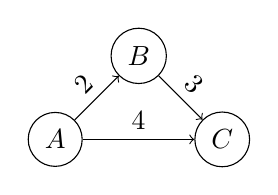
\begin{tikzpicture}[node distance = {15mm}, main/.style = {draw, circle}]
	\node[main] (1) {$A$};
	\node[main] (2) [above right of=1] {$B$};
	\node[main] (3) [below right of=2] {$C$};
	\draw[->] (1) -- (2) node[midway, above, sloped] {$2$};
	\draw[->] (2) -- (3) node[midway, above, sloped] {$3$};
	\draw[->] (1) -- (3) node[midway, above, sloped] {$4$};
\end{tikzpicture}
\end{center}

Then, since $w_{max} = 4$, $G'$ becomes

\begin{center}
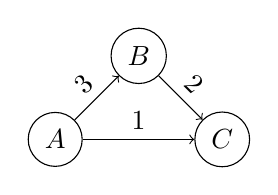
\begin{tikzpicture}[node distance = {15mm}, main/.style = {draw, circle}]
	\node[main] (1) {$A$};
	\node[main] (2) [above right of=1] {$B$};
	\node[main] (3) [below right of=2] {$C$};
	\draw[->] (1) -- (2) node[midway, above, sloped] {$3$};
	\draw[->] (2) -- (3) node[midway, above, sloped] {$2$};
	\draw[->] (1) -- (3) node[midway, above, sloped] {$1$};
\end{tikzpicture}
\end{center}

When we run Dijkstra's algorithm on $G'$, we notice that the shortest path in $G'$ is of length $1$, and according to the given algorithm, the longest path in $G$ should be the path corresponding to this cost, which is $A \to C$. However, the longest path in $G$ is $A \to B \to C$ instead, and this shows that the suggested algorithm is incorrect.

\end{solution}

\part[5] Recall that  a {\em Spanning Tree} of a given connected, weighted, undirected graph $G=(V, E)$ is a graph $G' = (V, E')$ with $E' \subseteq E$ such that $G'$ is a tree. The cost of a spanning tree is defined to be the sum of weight of its edges.
A {\em Minimum Spanning Tree (MST)} of a given connected, weighted, undirected graph is a spanning tree with minimum cost.
The following idea was suggested for finding an MST for a given graph in the class. 
\begin{quote}
Dijkstra's algorithm gives a shortest path tree rooted at a starting node $s$. Note that a shortest path tree is also a spanning tree. So, simply use Dijkstra's algorithm and return the shortest path tree.
\end{quote}
Show that the above algorithm does not necessarily output a MST.
In other words, a shortest path tree may not necessarily be a MST.
({\it For this question, you may consider only graphs with positive edge weights.})
\end{parts}

\vspace{0.2in}

\begin{solution}
Consider the graph obtained from removing the directedness of the edges of the graph considered in the previous part, i.e., let $G$ denote the following graph.
\begin{center}
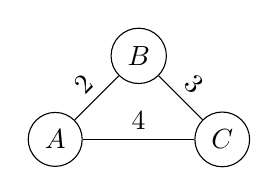
\begin{tikzpicture}[node distance = {15mm}, main/.style = {draw, circle}]
	\node[main] (1) {$A$};
	\node[main] (2) [above right of=1] {$B$};
	\node[main] (3) [below right of=2] {$C$};
	\draw[-] (1) -- (2) node[midway, above, sloped] {$2$};
	\draw[-] (2) -- (3) node[midway, above, sloped] {$3$};
	\draw[-] (1) -- (3) node[midway, above, sloped] {$4$};
\end{tikzpicture}
\end{center}

With the starting vertex as $A$, we see that the shortest path tree obtained from Dijkstra's algorithm has cost $6$, and is as follows:
\begin{center}
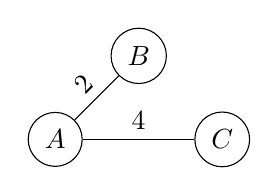
\begin{tikzpicture}[node distance = {15mm}, main/.style = {draw, circle}]
	\node[main] (1) {$A$};
	\node[main] (2) [above right of=1] {$B$};
	\node[main] (3) [below right of=2] {$C$};
	\draw[-] (1) -- (2) node[midway, above, sloped] {$2$};
	%\draw[-] (2) -- (3) node[midway, above, sloped] {$3$};
	\draw[-] (1) -- (3) node[midway, above, sloped] {$4$};
\end{tikzpicture}
\end{center}

However the following is a spanning tree with a smaller cost $5$:

\begin{center}
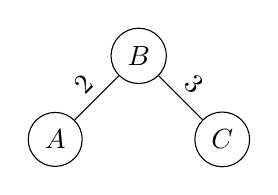
\begin{tikzpicture}[node distance = {15mm}, main/.style = {draw, circle}]
	\node[main] (1) {$A$};
	\node[main] (2) [above right of=1] {$B$};
	\node[main] (3) [below right of=2] {$C$};
	\draw[-] (1) -- (2) node[midway, above, sloped] {$2$};
	\draw[-] (2) -- (3) node[midway, above, sloped] {$3$};
	%\draw[-] (1) -- (3) node[midway, above, sloped] {$4$};
\end{tikzpicture}
\end{center}

This counterexample shows that the algorithm specified is incorrect.

We can also make a stronger claim. There exists a counterexample in which there is no source vertex such that the shortest path tree corresponding to running Dijkstra's algorithm from the vertex is a MST.

Consider the following graph:

\begin{center}
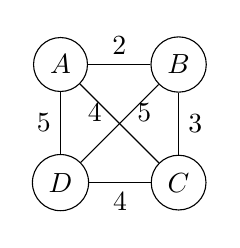
\begin{tikzpicture}[node distance = {15mm}, main/.style = {draw, circle}]
	\node[main] (1) {$A$};
	\node[main] (2) [right of=1] {$B$};
	\node[main] (3) [below of=2] {$C$};
	\node[main] (4) [left of=3] {$D$};
	\draw[-] (1) -- (2) node[midway, above] {$2$};
	\draw[-] (2) -- (3) node[midway, right] {$3$};
	\draw[-] (3) -- (4) node[midway, below] {$4$};
	\draw[-] (4) -- (1) node[midway, left] {$5$};
	\draw[-] (2) -- (4) node[midway, xshift=0.1cm, yshift=-0.1cm, above right] {$5$};
	\draw[-] (1) -- (3) node[midway, xshift=-0.1cm, yshift=-0.1cm, above left] {$4$};
\end{tikzpicture}
\end{center}

Consider the following spanning tree with cost $9$:

\begin{center}
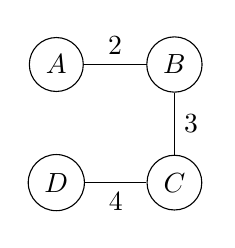
\begin{tikzpicture}[node distance = {15mm}, main/.style = {draw, circle}]
	\node[main] (1) {$A$};
	\node[main] (2) [right of=1] {$B$};
	\node[main] (3) [below of=2] {$C$};
	\node[main] (4) [left of=3] {$D$};
	\draw[-] (1) -- (2) node[midway, above] {$2$};
	\draw[-] (2) -- (3) node[midway, right] {$3$};
	\draw[-] (3) -- (4) node[midway, below] {$4$};
\end{tikzpicture}
\end{center}

If we run Dijkstra's algorithm from:

\begin{enumerate}
    \item $A$: cost 11
\begin{center}
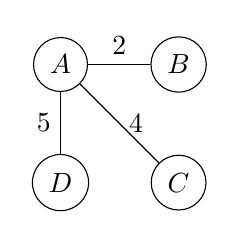
\begin{tikzpicture}[node distance = {15mm}, main/.style = {draw, circle}]
	\node[main] (1) {$A$};
	\node[main] (2) [right of=1] {$B$};
	\node[main] (3) [below of=2] {$C$};
	\node[main] (4) [left of=3] {$D$};
	\draw[-] (1) -- (2) node[midway, above] {$2$};
	\draw[-] (1) -- (3) node[midway, right] {$4$};
	\draw[-] (4) -- (1) node[midway, left] {$5$};
\end{tikzpicture}
\end{center}
    \item $B$: cost 10
\begin{center}
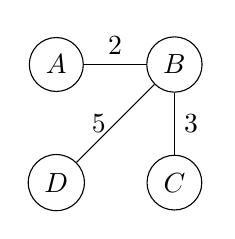
\begin{tikzpicture}[node distance = {15mm}, main/.style = {draw, circle}]
	\node[main] (1) {$A$};
	\node[main] (2) [right of=1] {$B$};
	\node[main] (3) [below of=2] {$C$};
	\node[main] (4) [left of=3] {$D$};
	\draw[-] (1) -- (2) node[midway, above] {$2$};
	\draw[-] (2) -- (3) node[midway, right] {$3$};
	\draw[-] (2) -- (4) node[midway, left] {$5$};
\end{tikzpicture}
\end{center}
    \item $C$: cost 11
\begin{center}
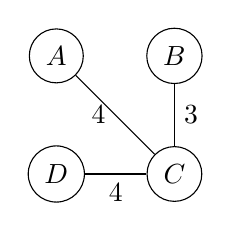
\begin{tikzpicture}[node distance = {15mm}, main/.style = {draw, circle}]
	\node[main] (1) {$A$};
	\node[main] (2) [right of=1] {$B$};
	\node[main] (3) [below of=2] {$C$};
	\node[main] (4) [left of=3] {$D$};
	\draw[-] (2) -- (3) node[midway, right] {$3$};
	\draw[-] (3) -- (4) node[midway, below] {$4$};
	\draw[-] (1) -- (3) node[midway, left] {$4$};
\end{tikzpicture}
\end{center}
    \item $D$: cost 14
\begin{center}
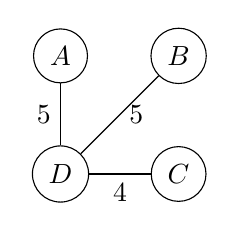
\begin{tikzpicture}[node distance = {15mm}, main/.style = {draw, circle}]
	\node[main] (1) {$A$};
	\node[main] (2) [right of=1] {$B$};
	\node[main] (3) [below of=2] {$C$};
	\node[main] (4) [left of=3] {$D$};
	\draw[-] (3) -- (4) node[midway, below] {$4$};
	\draw[-] (4) -- (1) node[midway, left] {$5$};
	\draw[-] (2) -- (4) node[midway, right] {$5$};
\end{tikzpicture}
\end{center}

\end{enumerate}

All of these costs are more than that of the spanning tree we found, and thus none of these are MSTs. 

\end{solution}

\question ({\it Example for ``greedy stays ahead"}) Suppose you are placing sensors on a one-dimensional road.  You have identified $n$ possible locations for sensors, at distances $d_1\le d_2 \le ...\le d_n$ from the start of the road, with $0 \leq d_1 \le M$ and $d_{i+1}-d_i \le M$.   You must place a sensor within $M$ of the start of the road, and place each sensor after that within $M$ of the previous one. The last sensor must be within $M$ of $d_n$.  Given that, you want to minimize the number of sensors used.  The following greedy algorithm, which places each sensor as far as possible from the previous one, will return a list $d_{i_1} \le d_{i_2} \le ... \le d_{i_k}$ of locations where sensors can be placed.  

\begin{framed}
{\tt GreedySensorMin($d_1...d_n, M$)}\\
\hspace*{0.1in} - Initialize an empty list\\
\hspace*{0.1in} - Initialize $I=1$, $PreviousSensor=0$.\\
\hspace*{0.1in} - While ($I < n$):\\
\hspace*{0.4in} - While ($I < n$ and $d_{I+1} \le PreviousSensor+ M$) $I++$\\
\hspace*{0.4in} - If ($I< n$) Append $d_I$ to list; $PreviousSensor=d_I$;$I++$. \\
\hspace*{0.1in} - if list is empty, append $d_n$ to list\\
\hspace*{0.1in} - return(list)
\end{framed}

In using the ``greedy stays ahead'' proof technique to show that
this is optimal, we would compare the greedy solution $d_{g_1},..d_{g_k}$ to another solution, $d_{j_1},..., d_{j_{k'}}$.
We will show that the greedy solution ``stays ahead'' of the other solution at each step in the following sense:\\
\underline{Claim}: For all $t \geq 1, g_t \geq j_t$.

\begin{parts}
\part[5]  Prove the above claim using induction on the step $t$.  Show base case and induction step.
\begin{solution}

We shall define a \textit{step} to be an iteration of the outer loop.

For convenience, we will define $g_0 = j_0 = 0$ and $d_0 = 0$.% meaning there is a supposedly a \emph{virtual} sensor at the start position 0 in any solution. 
This introduction will not change the substance of the claim above which is stated for $t \geq 1$ but as we will see this notational convenience will be useful in stating and proving the inductive hypothesis. Note that in the algorithm above the variable \texttt{previousSensor} is also initialized to 0.

\paragraph{Inductive Hypothesis} Let $P(t)$ : $g_t \geq j_t$, $t \in \{0 \ldots k\}$, and after the $t^\mathrm{th}$ step finishes, the value of $previousSensor$ is $d_{g_t}$.

\paragraph{Base Case:} $g_0 = j_0 = 0$ by construction, and since $previousSensor = 0 = d_{g_0}$ initially, the base case is trivially true.

\paragraph{Inductive Step:} Suppose that we have shown that $P(t-1)$ is true for some $t \ge 1$. We shall now show that this implies $P(t)$.
\begin{proof}
    If $g_t = n$ then the claim is trivially true as it is the last sensor that may be chosen. Therefore we will now suppose $g_t < n$.
    
    To begin, we shall first establish the following three inequalities.
    
    \begin{align}
        d_{j_t} &\leq d_{j_{t-1}} + M \\
        d_{g_t} &\leq d_{g_{t-1}} + M \\
        d_{g_t + 1} &> d_{g_{t-1}} + M
    \end{align}
    
    Equation (1) comes from the fact that for any valid solution $d_{j_0} \ldots d_{j_{k'}}$ to be valid it must satisfy the problem constraints which state that all sensors must be within a distance of $M$ of their nearest sensors.
    
    The proof for equations (2) and (3) comes from the algorithm as follows.
    
    We can see that in the solution, nothing between $g_{t - 1}$ and $g_{t}$ (both exclusive) has been appended to the list.
    
    Suppose there is an $I'$ such that $g_{t - 1} \le I' \le g_{t}$ and $d_{I'} > d_{g_{t - 1}} + M$.
    
    Consider the least such $I'$. Note that $g_{t - 1} \le g_{t - 1} + M$, so $I' \ne g_{t - 1}$, and thus $I' - 1 \ge g_{t - 1}$.
    
    Since $I'$ is the first such $I'$, we have $d_{I' - h} \le d_{g_{t - 1}} + M$ for all valid $h > 0$. This implies that in the iteration where $I = I' - 1$, we must have appended $d_{I' - 1}$ to the list, since $I' - 1 < N$ but $d_{I' - 1 + 1} > previousSensor + M$ and the internal while loop breaks at $I = I' - 1$.
    
    But since we have $g_{t - 1} \le I' - 1 < g_t$, we have appended either something between $d_{g_{t - 1}}$ and $d_{g_t}$ to the list (impossible by a previous observation), or $I' - 1 = g_{t - 1}$. This means $d_{g_{t - 1} + 1} > d_{g_{t - 1}} + M$, which is a contradiction to the given conditions (that between any two candidates for a position of the sensors, the distance is at most $M$).
    
    Hence, for all $I'$ such that $g_{t - 1} \le I' \le g_{t}$, we have $d_{I'} \le d_{g_{t - 1}} + M$.
    
    %We know that algorithm appended $d_{g_{t-1}}$ and $d_{g_t}$ into the solution list and no sensor in between, except for the special case of $t=1$, where although $d_0$ is not actually appended into the list, the variable $previousSensor$ still equals $0$.
    
    % replace step with moment
    % expand proof
    % I' first such
    
    %We can show that this implies that for all $I \in \{g_{t-1}, g_{t-1} + 1 \ldots g_t\}$, we have $d_I \leq d_{g_{t-1}} + M$ as $previousSensor = d_{g_{t-1}}$ during these steps and if there were a sensor $d_{I'}$ contradicting the claim, then at the $(I'-1)^{th}$ step the sensor $d_{I'-1}$ would have been appended into the solution list as constrained by the condition in inner while loop.
    
    This establishes equation (2).
    
    Since ${g_t} < n$, $g_t + 1 \le n$, hence $d_{g_t + 1}$ exists.
    Since $d_{g_t}$ was appended, from the termination condition of the inner loop of the algorithm at the step $I=g_t$ and the preceding sentence, equation (3) follows.
    
    Also, we have that when we append $d_{g_t}$, we set $previousSensor = d_{g_t}$.
    
    Now, since $P(t-1)$ holds, $j_{t-1} \leq g_{t-1} \implies d_{j_{t-1}} \leq d_{g_{t-1}}$. Substituting this inequality in equation (1) above we may as well obtain -
    \begin{align*}
        d_{j_t} &\leq d_{j_{t-1}} + M \leq d_{g_{t-1}} + M \\
        %\implies d_{g_{t-1}} &\geq d_{j_t} - M \\
    \end{align*}
    Finally, this inequality can be used in equation (3) to reach the final conclusion -
    \begin{align*}
        \implies d_{g_t + 1} &> d_{g_{t - 1}} + M \ge d_{j_t} \\
        \implies g_t + 1 &> j_t \quad\text{\Comment{as $d$ is a non-decreasing sequence}}\\
        \implies g_t &\geq j_t
    \end{align*}
    And thus the inductive step is complete and the hypothesis is established.
\end{proof}
\end{solution}

\part[3] Use the claim to argue that $k' \geq k$. (Note that this completes the proof of optimality of the greedy algorithm since it shows that greedy algorithm places at most as many sensors as any other solution.)
\begin{solution}
We shall prove this claim using proof by contradiction. Suppose there exists a solution such that $k > k'$. $k'$ can not be 0 as one sensor has to be placed. Then we have
\setcounter{equation}{0}
\begin{align}
    d_{j_{k'}} &\geq d_n - M \\
    d_{g_{k'}} &\geq d_{j_{k'}}
\end{align}
Equation (1) follows from the problem constraints that state that for any solution to be valid, the last sensor must be within a distance of $M$ of $d_n$. Equation (2) follows from the claim established in the previous part of this problem. These 2 results will together yield
\[
    d_{g_{k'}} \geq  d_n - M
\]
But once the algorithm appends $d_{g_{k'}}$ to the solution list then for all $I$ such that $g_{k'} < I < n$ the algorithm will never append $d_I$ to the solution list because $I < n$ \textbf{and} $d_{I+1} \leq d_n \leq d_{g_{k'}} + M$ so the inner loop constraint will always be satisfied and both the loops will terminate. This shows that the greedy solution will also place no more than $k'$ sensors and thus $k \leq k'$ which is a contradiction to supposition.
\end{solution}

\part[2] In big-O notation, how much time does the algorithm as written take? Write a brief explanation.
\end{parts}
\begin{solution}
We observe that the variable $I$ is initialized to $0$ at the start of program and then the only operation performed on it is the increment by one operation which is performed per iteration of both the loops in the algorithm. Both the loops of the algorithm terminate when $I$ reaches $n$ therefore $I$ may only be increment $n$ times. This also shows that \textbf{both} the loops may execute for a total of $O(n)$ iterations in the entire duration of algorithm, this means that there may be $O(n)$ append operations, assuming each append operations takes $O(1)$ steps (either amortized or otherwise) we can conclude that the total run time complexity of the algorithm is $O(n)$.
\end{solution}



\vspace{0.3in}








\question ({\it Example for ``modify the solution"})
You have $n$ cell phone customers who live along a straight highway, at distances $D[1] < D[2] <  ... < D[n]$ from the starting point.  
You need to have a cell tower within $\Delta$ distance of
each customer, and want to minimize the number of cell towers.  

({\it For example, consider $\Delta=3$ and there are $3$ customers  (i.e., $n = 3$) with $D[1] = 3, D[2] = 7, D[3] = 10$}. In this case, you can set up two cell towers, one at $6$ and one at $10$.)

Here is a greedy strategy for this problem.
\begin{quote}
{\bf Greedy strategy}: Set up a tower at distance $d$ which is at the farthest edge of the connectivity range for the customer who is closest to the starting point. That is, $d = \Delta + D[1]$. Note that all customers who are within $\Delta$ distance of this tower at $d$, are covered by this tower. 
Then recursively set up towers for the remaining customers (who are not covered by the first tower).
\end{quote}

We will show that the above greedy strategy gives an optimal solution using modify-the-solution. For this, we will first need to prove the following exchange lemma.

\underline{\it Exchange Lemma}: {\it Let $G$ denote the greedy solution and let $g_1$ be the location of the first cell phone tower set up by the greedy algorithm. Let $OS$ denote any solution that does not have cell phone tower at $g_1$. Then there exists a solution $OS'$ that has a cell phone tower set up at $g_1$ and $OS'$ has the same number of towers as $OS$.}

\underline{\it Proof.} Let $OS = \{o_1, ..., o_k\}$. That is, the locations of the cell phone towers as per solution $OS$ is $o_1 < o_2 < ... < o_k$. We ask you to complete the proof of the exchange lemma below.

\begin{parts}
\part[1] Define $OS'$.
\begin{solution}

Remove all the towers (if any) which are at distance less than  or equal to $g_{1}$ from the starting point, and add a tower at $g_{1}$, where $g_{1}$ is the greedy choice of the location of the first tower i.e. $\Delta + D[1]$.

Formally, let $q$ be the last tower in $OS$ such that $o_q \le g_1$.

If such a $q$ exists, then define
$$OS'= OS - \{o_1, \ldots, o_{q}\} \cup \{g_1\} = \{g_{1}, o_{q + 1}, \ldots, o_k\}$$

Else define
$$OS'= OS \cup \{g_1\} = \{g_{1}, o_1, \ldots, o_k\}$$

Note: we will show that the second case never arises, and this definition is given only for the sake of covering all the possible cases at this point.
\end{solution}

\part[2] $OS'$ is a valid solution because... ({\it justify why $OS'$ provides coverage to all customers.})
\begin{solution}

Let us assume there exist a person $i$ that does not get the signal in $OS'$ but gets the signal in $OS$ (as it is valid solution).

Therefore there exists a $j$ s.t. $|D[i]-o_{j}| \leq \Delta$. \Comment{As OS is a valid solution}

Let $q$ be the last tower whose distance is at most $g_{1}$ if it exists.

\textbf{Case 1}: $q$ exists and $j \le q$.

$$|D[i]-o_{j}| \leq \Delta$$
$$\implies \Delta-o_{j} \leq D[i] \leq o_{j}+\Delta$$

We have the fact that $o_{j} \leq o_{q} \leq D[1] + \Delta$, so we have

$$D[i] \leq D[1]+2\Delta$$

As $D$ is sorted in ascending order, therefore,

$$D[1] \le D[i]$$ 

Combining both we get

$$D[1] \le D[i] \leq D[1]+ 2\Delta$$
$$\implies |D[i]-(D[1]+\Delta)| \leq \Delta$$

As our greedy strategy takes $g_1 = D[1]+\Delta$ as its first choice. Therefore,

$$|D[i]-g_1| \leq \Delta$$

Therefore this $i^\mathrm{th}$ person will get coverage in $OS'$ and we don't get any $i$ in this case satisfying our assumption.

\textbf{Case 2}: $q$ exists and $j > q$.

As $o_{j}$ is still in the $OS'$ therefore the same tower will provide the customer $i$ its coverage.

In this case also there is no $i$ satisfying our assumption.

\textbf{Case 3}: $q$ does not exist.

In this case, each $o_r$ satisfies $o_r > g_1$. This means that $o_r - D[1] > g_1 - D[1] = \Delta$, so the first customer is not covered by any tower in $OS$, which is a contradiction to the assumption that $OS$ was a valid solution.

So, there is no such $i$ in this case either.

As Case 1, 2, 3 are disjoint and mutually exhaustive therefore there does not exist any such customer $i$ which satisfies our assumption.

This is a contradiction and hence $OS'$ provides coverage to all customers.

\end{solution}

\part[2] The number of cell phone towers in $OS'$ is at most the number of cell phone towers in $OS$ because... ({\it justify})
\end{parts}
\begin{solution}

In the algorithm we have removed all the towers (if any) whose distance are less than $g_{1}$ and added the tower at $g_{1}$. 

Therefore to prove that the number of cell phone towers in $OS'$ is at most $OS$, it is sufficient to prove that there exists at least one tower in $OS$ whose distance is at most $g_{1}$.

As $OS$ is a valid solution then $D[1]$ also gets the coverage. Therefore, there exists $j$ such that $ |D[1]-o_{j}| \leq \Delta$. Therefore, $o_{j} \leq D[1]+\Delta$.

Hence, there exists at least one tower in $OS$ whose distance is at most $g_1$, as needed.


\end{solution}
We will now use the above exchange lemma to argue that the greedy algorithm outputs an optimal solution for any input instance. 
We will show this using mathematical induction on the input size (i.e., number of customers). The base case for the argument is trivial since for $n=1$, the greedy algorithm opens a single tower which is indeed optimal.

\begin{parts}
\part[3] Show the inductive step of the argument.
\end{parts}

\begin{solution}
Here, we assume that the greedy algorithm outputs an optimal solution for all inputs with $k$ customers where $1 \leq k \leq n - 1$. We will show that the greedy algorithm outputs an optimal solution for any input with $n$ customers. 

Let $GS(P)$ denote the greedy solution for the instance of problem $P$.

Let $P$ be a problem instance with $n$ customers.
We can write $GS(P) = g_{1} \cup GS(P')$ where the first tower is placed at $g_{1}$ as per the greedy choice and $P'$ is the problem instance with the customers who are not in the range of the first tower, having $n'$ customers.

Let $OS(P)$ be any arbitrary solution for the problem $P$.

Then by exchange lemma we can find $OS'(P)$ such that the first tower is at $g_{1}$ and $|OS'(P)| \leq |OS(P)|$. where $|.|$ denotes the number of mobile towers. So we may write $OS'(P) = g_{1} \cup OS''(P')$, where $OS''(P')$ is the remaining part of the solution $OS'(P)$. Note that $OS''(P')$ is a valid solution for $P'$ since when we remove the first tower, we remove all customers in its range, so for any other customer in $P'$, it must have another tower (which is not at $g_1$) serving that customer, as $OS'(P)$ is valid.
Then we have,

\begin{align*}
    |GS(P)| &= 1 + |GS(P')|\\
          &\leq 1 + |OS''(P')|\\
          &= |OS'(P)|\\
          &\leq |OS(P)|
\end{align*}

Here the first inequality comes from the induction hypothesis as $n'$ is less than $n$.

So the greedy solution is as good as any other solution and hence optimal.
\end{solution}



Having proved the correctness, we now need to give an efficient implementation of the greedy strategy and give time analysis.


\begin{parts}
\part[5] Give an efficient algorithm implementing the above strategy, and give a time analysis for your algorithm.
\end{parts}
\begin{solution}
\begin{algorithmic}[1]
\Function{greedyTowers}{$D[1\ldots n]$}
\State let $towers \gets$ empty list
\State let $k \gets 1$
\While {$k \leq n$}
    \State $curr\_tower \gets D[k] + \Delta$
    \State insert $curr\_tower$ into $towers$
    \While {$k \leq n$ and $D[k] \leq curr\_tower$}
        \State $k \gets k + 1$
    \EndWhile
\EndWhile
\State \Return $towers$
\EndFunction
\end{algorithmic}

\textbf{Running Time Analysis}

%Suppose the outside loop runs $p$ times where $p \leq n$ %and in that corresponding inside loop run at $a_{i}$ times where $\sum_{i=1}^{p} a_{i} = n$ and  $a_{i} \geq 1$.

Note that at each iteration of the inside loop, we increment $k$ by $1$. Since we break when $k$ exceeds $n$, the inner loop runs exactly $n$ times.

Since we have $\Delta \ge 0$, we have $D[k] \le curr\_tower$ after line $5$. Also, we have $k \le n$ by the if-condition, and thus, the inner loop runs at least once for each iteration of the outer loop. Hence, the outer loop runs at most $n$ times.

Note that in each iteration of the outer loop, ignoring the inner loop, we do $O(1)$ work, and in each iteration of the inner loop, we do $O(1)$ work too. Hence the total time taken by the outer loop over the whole execution of the program is $O(\# \text{total iterations of the outer loop in the program} + \# \text{total iterations of the inner loop in the program}) \in O(n)$.

Initialising a list and $k$ takes constant time, and returning the list takes $O(k)$ time, which is in $O(n)$.

%Time take for the ith iteration of outside of the while loop will be O(1) + O($a_{1}$). Taking sum for all i it will translate into O(p+n) which is same as O(n) as p$\leq$n
Therefore the time complexity of complete algorithm will be $O(n)$.

\end{solution}



\vspace{0.4in}

\question[25] You are a conference organiser and you are asked to organise a conference for a company. 
The capacity of the conference room is limited and hence you would want to minimise the number of people invited to the conference.
To make the conference useful for the entire company, you need to make sure that if an employee is not invited, then every employee who is an immediate subordinate of this employee gets the invitation
({\it if an employee is invited, then you may or may not invite a subordinate}).
The company has a typical hierarchical tree structure, where every employee except the CEO has exactly one immediate boss.

Design an algorithm for this problem. You are given as input an integer array $B[1...n]$, where $B[i]$ is the immediate boss of the $i^{th}$ employee of the company. The CEO is employee number $1$ and $B[1]=1$. The output of your algorithm is a subset $S \subseteq \{1, ..., n\}$ of invited employees. 
Give running time analysis and proof of correctness.

\begin{solution}

%We begin by the discussion of the corner case of the problem.
%\paragraph{Important note regarding corner cases} Note that the problem statement is slightly ambiguous in the case when there is only one employee in the company - the CEO. If we are to follow the problem constraints strictly, then vacuously, it is not necessary to invite the CEO. In that case, we can get rid of lines 15-17 in the algorithm to get the answer as an empty set, and the inductive proof would work fine too. However, from another perspective, for the conference to be useful for the company, at least one employee needs to attend the conference. This ambiguity leads us to consider two different versions of the problem. We claim that the only corner case is $n = 1$, i.e., for $n > 1$, we will always have at least one employee in the conference if we enforce only the condition in the problem statement (hence this shows that apart from the case $n = 1$, the conditions are equivalent). Indeed, suppose there is no employee invited. In particular, the CEO is not invited. Since $n > 1$, the CEO must have at least 1 subordinate, who must be invited, which is a contradiction. So the only corner case is $n = 1$, whose analysis has been done above already. Hence, we will only focus on the case where $n > 1$ in the following analysis of the problem, since we have handled the case $n = 1$ here already.

In the greedy algorithm described below, we make a decision for each employee -- whether that employee should be invited or not.

To make such a greedy assignment feasible, we first arrange the employees linearly in a suitable fashion; for our algorithm, this suitable fashion is the topologically sorted array of graph $G$ where there is an edge from $v$ to $u$ if and only if $u$ is the immediate boss of $v$ (it is the reverse graph of the arborescence induced by the boss-subordinate relation, with the CEO at the root).%formed by boss-subordinate relation of the employees.

The topological sorting is done so that the subordinates come before their boss in the array (thus, one can imagine edges from subordinates to their boss). Once arranged in this linear fashion we make a decision of each employee, the decision is represented in the algorithm by a boolean variable -- True indicating that the employee should be invited and False if the employee better not be invited.

Intuitively we first decide not to invite any employees at all and then at each step we make a decision, we invite the current employee's boss iff the employee is marked False. We shall later prove in the proof of correctness that such a greedy decision assignment is indeed the optimal one.

\begin{algorithmic}[1]
    \Function{Problem5}{$B[1\ldots n]$}
        \State let $G \gets$ array of size $n$ of (empty) adjacency lists.
        \For{$i \in [2 \ldots n]$}
            \State Append $B[i]$ into $G[i]$ 
        \EndFor
        \State let employees $\gets$ \Call{TopoSort}{$G$}
        \State let mapping $\gets \{ \text{employees}[i] \mapsto i \; \forall i \in [1 \ldots n] \}$
        \State decision $\gets$ boolean array of size $n$ initialized to all false.
        \For{$i \in [1 \ldots n]$}
            \State let $e \gets$ employees$[i]$
            \If{decision[$i$] is False and $B[e] \ne e$}
                \State decision[$mapping[B[e]]$] $\gets$ True
            \EndIf
        \EndFor
        \State let ans $\gets$ empty set.
        \For{$i \in [1 \ldots n]$}
            \State let $e \gets$ employees$[i]$
            \If{decision[$i$] is True}
                \State add $e$ to ans
            \EndIf
        \EndFor
        \State \Return ans
    \EndFunction
\end{algorithmic}

\paragraph{Proof Of Correctness}
We adopt the notation of representing a solution as a sequence of boolean decisions one for each employee of whether that employee should be invited or not. In particular in this list of decisions the employees appear in order as specified by the variable \texttt{employees} in the pseudocode. The variable \texttt{decisions} in the pseudo-code above is based on this convention only.

First we need to show that the greedy solution is consistent with the problem constraints. To show that we will prove a number of useful lemmas.

\begin{lemma}
For any 2 employees $e_1$ and $e_2$, if $e_1$ is a (direct or indirect) subordinate of $e_2$ then $e_1$ comes before $e_1$ is the ordering of decisions imposed by the variable \texttt{employees} in the psuedocode.
\end{lemma}
\begin{proof}
    In the pseudocode we can notice that the graph $G$ is constructed (in adjacency list representation) such that there is an edge from $u$ to $v$ \emph{iff} $u$ is a direct subordinate of $v$. This is because for every employee $u$ (except CEO), we insert the edge $(u,B[u])$ in $G$ at the $u$th iteration of the first loop in algorithm. Therefore $G$ has only edges from subordinates to their boss. Clearly, $G$ is also acyclic as laid down by the problem constraints. Then, by the properties of topological sorting studied we know that in the topological order \texttt{employees} of employees the subordinates must come before their boss as in a topologically sorted array, for each edge $(u, v)$, $v$ comes after $u$ in the array.
\end{proof}
The lemma proved above is fundamental to proving the correctness of our greedy algorithm because it defines the precise ordering of the sequence of decisions made by the greedy algorithm -- subordinates first. This ordering will also be useful in proving the optimality of the greedy algorithm later.

\begin{lemma}
If the greedy algorithm makes a decision of True for an employee $e$. Then it must have made the decision of False for at least one of its subordinates.
\end{lemma}
\begin{proof}
We can note that the array \texttt{decisions} is initially initialized to all False and then from the loop at line 9 of the algorithm a decision is only converted to True if there is a employee $x$ that comes before employee $e$ in the ordering \texttt{employees} such $e$ is the boss of $x$ and $x$ has been given the decision False.
\end{proof}
%We would emphasize that the above lemma does not hold when the CEO is the only employee as we have explicity handled the case in the algorithm. This is because the problem constraints which say $B[1]=1$ mandate that in such an exceptional case the CEO -- the only employee must be invited to the meeting even though technically \emph{none} of its subordinates are uninvited. 

\begin{lemma}
If the greedy algorithm makes a decision of False for an employee $e$. Then it must have made the decision of True for all its subordinates.
\end{lemma}
\begin{proof}
Suppose $x$ is a direct subordinate of $e$ such that the algorithm makes the decision of False for $x$. Note that $x$ will come before $e$ in the ordering \texttt{employees}. Therefore, from loop 2 of the algorithm we can see that since $x$ has been marked as False, the boss of $x$ (which is $e$) will be marked True. Therefore we can conclude that if an employee is not marked True then it must have had no employees marked False.
\end{proof}
The last lemma proves that the decision made by greedy algorithm is at least consistent with problem constraints as either an employee $e$ will be invited or all of its sub-ordinates will be invited. Note however that in the lemma established previous to this one we also showed that when an employee is invited at least one of its subordinates must be un-invited. Although this is not mandated by problem constraints as it is allowed for both bosses and all their sub-ordinates to be invited together, the greedy algorithm places this constraint \emph{because} the decision made by greedy algorithm is not just any consistent solution but, as we shall prove later, one of the optimal consistent solutions. We shall now turn to the proof of this optimality.

We shall prove the optimality of our greedy algorithm using the \emph{proof by exchange} technique. Now suppose $S$ be \emph{the} solution (decisions) made by our greedy algorithm above. Then we state for all $i \in [1 \ldots n]$ -

\paragraph{Induction Hypothesis:} $P(i)$: Let $O$ be any (not necessarily optimal) sequence of decisions, then there exists a transformed valid solution $O'$ corresponding to $O$ such that $O'[1 \ldots i] = S[1 \ldots i]$ and $O'$ is at least as good as $O$.

\paragraph{Base Case:} When $i = 0$, we can trivially set $O' = O$. The validity of $O'$ comes from the validity of $O$, and the number of people invited to the conference is the same, hence completing proof of the base case.%When $i=1$. Note that the employee $e = \texttt{employees}[1]$ has no sub-ordinates as we have already established from the property of \texttt{employees} ordering. Therefore our greedy algorithm will never make a decision of True for this employee $e$ \emph{except} when $e$ is the only employee -- CEO. Now, suppose $O$ is some solution such that $O[1]=$ True. If $e$ is CEO then the greedy algorithm makes the same decision therefore we have $O'=O$. Otherwise, we can construct $O'$ from $O$ by making the following transformation: Set $O[1]=$ False and $O[x]=$ True where $x: $ employees$[x]$ = $B[e]$. In algorithmic terms it is $x = mapping[B[e]]$.

%Note that if $O[1]$ was originally False, then $O[x]$ must have been True to make $O$ consistent. If $O[1]$ was originally True, then $O[x]$ could have been either True or False, and in this case, we have 

Such a transformation will preserve consistency and is at least as good as $O$. Therefore we have found the desired solution $O'$.

\paragraph{Inductive Step:} Suppose we have already shown $P(i-1)$ holds for some $i \in [1 \ldots n]$. We will now prove that this implies that $P(i)$ also holds.

Since $P(i-1)$ holds, we have that there exists a transformed valid solution $O'$ such that $O'[1 \ldots i-1] = S[1 \ldots i-1]$ and $O'$ is at least as good as $O$. So we can simply show that $O'$ can again be transformed into some valid solution $O''$ such that $O''[1 \ldots i] = S[1 \ldots i]$ and $O''$ is at least as good as $O'$ to prove the implication. So we shall focus on $O'$. Three cases arise -

\begin{enumerate}
    
    \item $O'[i] = S[i]$. In this case we can set $O'' = O'$ and we are done trivially.
    
    \item $S[i] =$ True but $O'[i] =$ False. That is, the greedy algorithm made the decision of invitation for employee $e=$ employees$[i]$ but the solution $O'$ decided not to invite $e$. In this case we shall show that such a solution $O'$ is not valid, which would be a contradiction.
    
    Consider $e$ and its direct sub-ordinates $\{x_1, \ldots, x_k\}$ (maybe empty set). We have shown already that if our greedy algorithm makes the decision of True for a employee then it must have also made the decision of False for at least one of its subordinates. Let $x$ be that subordinate. We have also shown that $x$ must come before $e$ in the ordering of decisions, and since $O'[1 \ldots i-1] = S[1 \ldots i-1]$ we have that the solution $O'$ also makes the (same) decision of False for employee $x$. Note that this implies that $O'$ made the decision of False for both $x$ and its boss $e$ here, which violates the problem constraints and thus no such valid solution $O'$ may exist. This case is therefore impossible.
    
    \item $S[i] =$ False but, $O'[i] =$ True. That is, the greedy solution decided not to invite the employee $e=$ employees$[i]$ but the solution $O'$ decided otherwise.
    
    In this case, consider the transformed solution $O''$ formed from $O'$ by following transformation: Set $O'[i]$ = False and $O'[x] =$ True where $x$ is such that employees$[x]=B[e]$ (in algorithmic terms it is $x = mapping[B[e]]$). We do not do the second assignment if $x = i$, i.e., $e$ is the CEO.
    
    Note that the solution $O''$ is at least as optimal as $O'$ because we un-invited an employee $e$ and we are inviting at most one additional employee -- $e$'s boss if it exists. So, total number of invited employees will either remain same or decrease by one.
    
    Now we only need to show that $O''$ is indeed a valid sequence of decisions which do not invalidate the problem constraints. Note that a change in decision of employee $e$ can only cause inconsistencies with decisions of its subordinates or one of its superiors.
    
    First, consider $e$ and its subordinates $\{x_1, \ldots, x_k\}$. We have already shown that if our greedy algorithm decides on a False for employee $e$ then it must have decided on True for all its subordinates $\{x_1, \ldots, x_k\}$. And since all the subordinates come before the employee $e$ in ordering of sequence of decisions, we can conclude that the solution $O'$ will also decide on inviting all the subordinates $\{x_1, \ldots, x_k\}$ as $O'[1 \ldots i-1] = S[1 \ldots i-1]$. Therefore not inviting the employee $e$ will not cause any inconsistencies in decisions of $e$ and its subordinates.
    
    Now we turn our attention to $B[e]$ -- the boss of $e$ (if the boss exists, i.e., if $e$ is not the CEO). Since in our transformation we are setting $O'[x]=$ True, this means that the employee $B[e]$ can not have a inconsistency anymore from un-invitation of $e$ as $B[e]$ itself is invited. Also, since $B[e]$ is now coming to the conference, the boss of $B[e]$ (if it exists) can either come or not come, and hence the original decision regarding it is consistent. Therefore, we have shown that the sequence of decisions $O''$ is still consistent with the problem constraints, and $O''$ is at least as good as $O'$ which is at least as good as $O$.
\end{enumerate}
Therefore, for all the cases we have shown that the implication $P(i-1) \implies P(i)$ holds. Thus, the induction is established.

From the induction hypothesis above, the optimality of greedy algorithm is also established. As, if $O$ is any true optimal solution then the hypothesis establishes that $O$ may be transformed to an at least as good solution $O'$ such that $O'[1 \ldots n] = S[1 \ldots n]$. Therefore the greedy solution is at least as good as any other optimal solution, and hence must be optimal itself.

\paragraph{Running Time Analysis} Firstly, we construct a graph $G$ representing boss-subordinate relations. Initializing the array of empty adjacency lists will take $O(n)$ time. Each employee has exactly one boss, and therefore the first loop in the pseudocode will run exactly $n-1$ times therefore taking $O(n)$ steps. We know that \texttt{TopoSort} subroutine takes $O(V+E)$ time. Here, $V = O(n)$ and $E = O(n)$ as each employee has at most one boss. Therefore topo sort will also take $O(n)$ steps. Then we create a mapping which maps each employee to its position in the toposorted array. To construct this mapping we can simply iterate through the \texttt{employees} array and do the specified assignment ($mapping[employees[i]] = i$). So this step will also take $O(n)$ time. Finally we initialize the array \texttt{decision} which takes $O(n)$ steps still and we again iterate once through the \texttt{employees} taking $O(n)$ steps. Finally we iterate through \texttt{decision} and in each iteration we potentially insert a element into the \texttt{ans} set. Assuming set insertion (implementing a set as a list) takes $O(1)$ time, the total time taken for this loop will also be $O(n)$. All the remaining operations such as return statements take only $O(1)$ time (assuming return by reference, else $O(n)$). Therefore we can conclude that the algorithm completes overall in linear time -- $O(n)$.
\end{solution}


\vspace{0.4in}


\question[25] A town has $n$ residents labelled $1, ..., n$. In the midst of a virus outbreak, the town authorities realise that hand sanitiser has become an essential commodity. 
They know that every resident in this town requires at least $T$ integer units of hand sanitiser. 
However, at least $\lceil \frac{n}{2}\rceil$ residents do not have enough sanitiser. 
On the other hand, there may be residents who may have at least $T$ units. 
With very few new supplies coming in for the next few weeks they want to implement some kind of sharing strategy. 
At the same time, they do not want too many people to get in close proximity to implement sharing. So, they come up with the following idea:
\begin{quote}
Try to {\em pair up} residents (based on the amount of sanitiser they possess) such that: 
\begin{enumerate}
\item A resident is either unpaired or paired with exactly one other resident. 
\item Residents in a pair together should possess at least $2T$ units of sanitiser.
\item The number of unpaired residents with less than $T$ units of sanitzer is minimised.
\end{enumerate}
\end{quote}

Once such a pairing is obtained, the unpaired residents with less than $T$ units of sanitiser can be  managed separately. The town authorities have conducted a survey and they know the amount of sanitiser every  resident possesses. You are asked to design an algorithm for this problem. You are given as input integer $n$,  integer $T$, and integer array $P[1...n]$ where $P[i]$ is the number of units of sanitiser that resident $i$ possesses. You may assume that $0 \leq P[1] \leq P[2] \leq ... \leq P[n]$. 
Your algorithm should output a pairing as a list of tuples $(i_1, j_1), (i_2, j_2), ..., (i_k, j_k)$ of maximum size such that (i) For all $t = 1, ..., k$, $P[i_t] + P[j_t] \geq 2T$ and (ii) $i_1, ..., i_k, j_1, ..., j_k$ are distinct.
Give proof of correctness of your algorithm and discuss running time.

\begin{solution}

\setcounter{lemma}{0}
\setcounter{claim}{0}


Note that the problem asks in point 3 to minimise the number of unpaired residents with less than $T$ units of sanitizer (i.e., maximize the number of paired residents with less than $T$ units of sanitizer), however later in the problem statement, we are asked to maximize the size of the pairing. So, we exhibit an algorithm which maximizes both the size of the pairing as well as the number of paired residents with less than $T$ units of sanitizer.

\vspace{0.5cm}

\textbf{Algorithm:}


\begin{algorithmic}[1]
    \Function{Problem6}{$n, T, P[1 \dots n]$}
        \State let $\mathit{pairings}$ = empty list
        \State let $l = 1$
        \State let $r = n$
        \While{$l < r$}
            \If{$P[l] + P[r] \ge 2T$}
                \State append $(l, r)$ to $\mathit{pairings}$
                \State $r \gets r - 1$
            \EndIf
            \State $l \gets l + 1$
        \EndWhile
        \State \Return $\mathit{pairings}$
    \EndFunction
\end{algorithmic}

\vspace{0.5cm}

\textbf{Proof of correctness:}

\begin{claim}
The following greedy strategy works:\nl
For the rightmost unassigned resident with the largest $P-$value $x$, we try to find the leftmost unassigned resident with the least $P-$value $y$ satisfying $x + y \ge 2T$. Call such a pair of residents a \textbf{nice} pair of residents.\\
If we cannot find any such resident, we return an empty list. Else, we pair these residents (with the first resident on the right), add them to the list, remove them from consideration and recursively find the answer for the remaining residents, and concatenate the answer to that instance with our list, and return it.\\
(Note that since $P$ is sorted, the rightmost unassigned element also has the maximum $P$ value, and similarly, the leftmost unassigned resident satisfying the condition above is also a resident with the least $P$ value satisfying the condition).
\end{claim}
\begin{proof}
Define $v(S) =$ number of pairs in a solution $S$ to the problem, and $u(S) =$ number of paired residents with $< T$ units of sanitizer.
\begin{lemma}
For any solution $OS$ with $v(OS) > 0$, there exists another solution $OS'$ with a nice pair of residents which has $v(OS') \ge v(OS)$ as well as $u(OS') \ge u(OS)$.
\end{lemma}
\begin{proof}
Let $M$ be the rightmost resident (with the largest $P$ value).\nl
Firstly note that if $v(OS) > 0$, there exists at least one pair of residents $i, j$ which have $P[i] + P[j] \ge 2T$. Note that if such a pair exists, we have, by the definition of $M$, that $P[M] + P[j] \ge P[i] + P[j] \ge 2T$, so the set of all residents $r$ which satisfies $P[M] + P[r] \ge 2T$ is non-empty.\nl
Let resident $m$ be a resident with the least $P$ value in the above set.\nl
If $(m, M)$ are paired in $OS$, we can take $OS = OS'$ and we will be done. Now assume that this is not the case. We make cases on which of $m, M$ are assigned in $OS$.
\begin{enumerate}
    
    \item Neither of $m, M$ are assigned:\nl
    In this case, we can simply pair them up to get $OS' = (m, M) \cup OS$ (which is valid by the definition of $m$, the validity of $OS$ and the disjoint nature of all pairs in the pairing) to get $v(OS') = v(OS) + 1 > v(OS)$. Note that since we are only inserting a pairing, we have $u(OS') \ge u(OS)$.
    
    \item $m$ is assigned to some $M'$ but $M$ is unassigned\nl 
    In this case we know that $P[m] + P[M] \ge 2T$, so the solution $OS' = \left(OS - \{(m, M')\}\right) \cup (m, M)$ is a valid solution (by the definition of $m$, the validity of $OS$ and the disjoint nature of all pairs in the pairing), and we have $v(OS') = v(OS)$.\nl
    Note that since $m, M'$ are paired, we have $P[m] + P[M'] \ge 2T$. 
    
    Firstly we claim that $m$ is to the left of $M'$. Suppose that this is not the case. Then we have $m$ to the left of $M$ since $M$ is the rightmost resident. So we have $P[m] \le P[M]$. Then we have $P[M'] + P[M] \ge P[M'] + P[m] \ge 2T$. Now by assumption, $M'$ is to the left of $m$, so $m$ is no longer the leftmost resident to satisfy the property that $P[M] + P[m] \ge 2T$.
    
    So $m$ is to the left of $M'$. Now if $P[m] \ge T$, we have $P[M'] \ge T$ as well as $P[M] \ge T$, so in this case $u(OS') = u(OS)$. Else, we have $P[m] < T$, so since $P[m] + P[M'] \ge 2T$, we have $P[M'] \ge T$, and similarly, $P[M] \ge T$. So in this case too, $u(OS') = u(OS)$.
    
    \item $M$ is assigned to some $m'$ but $m$ is unassigned\nl
    In this case we know that $P[m] + P[M] \ge 2T$, so the solution $OS' = \left(OS - \{(m', M)\}\right) \cup (m, M)$ is a valid solution (by the definition of $m$, the validity of $OS$ and the disjoint nature of all pairs in the pairing), and we have $v(OS') = v(OS)$.
    
    Note that $m$, by definition, is to the left of $m'$, since $m$ is the leftmost resident to satisfy $P[M] + P[m] \ge 2T$. In the case that $P[m'] < T$, we also have $P[m] < T$, so $P[M] \ge T$, and in this case $u(OS') = u(OS)$. In the case that $P[m'] \ge T$, we can either have $P[m] < T$ or $T \le P[m] \le P[m']$. In the former case, $u(OS') = u(OS) + 1$, and in the latter, $u(OS') = u(OS)$.
    
    \item $M$ is assigned to $m'$ and $m$ is assigned to $M'$: in this case, we see that since $m$, by definition, has the least $P$ value of any resident that can be assigned to $M$, $P[m'] \ge P[m]$. So we have $P[M'] + P[m'] \ge P[M'] + P[m] \ge 2T$ where the second inequality comes from $m$ being paired with $M'$ validly. Also, we have $P[M] + P[m] \ge 2T$ by the definition of $m$. So the solution $OS' = \left(OS - \{(m, M'), (m', M)\}\right) \cup \{(m, M), (m', M')\}$ is a valid solution (by the argument above, the validity of $OS$ and the disjoint nature of all pairs in the pairing), and $v(OS') = v(OS)$.
    
    Note that since we only rearrange already existing pairings, the number of paired residents with $< T$ units of sanitizer is preserved, and in this case, we have $u(OS') = u(OS)$.
    
\end{enumerate}
In all the above cases, we have shown that there exists a solution $OS'$ in which $m, M$ are paired and $v(OS') \ge v(OS)$ as well as $u(OS') \ge u(OS)$, which concludes the proof of the lemma.
\end{proof}
Now we induct on the number of residents to show that for any solution $S$ to any instance of the problem, the greedy solution $G$ for that instance satisfies $v(G) \ge v(S)$ as well as $u(G) \ge u(S)$.

\textbf{Inductive hypothesis:} Let $P(n)$ be the assertion that for any solution $S$ to an instance of the problem with $n$ residents, the greedy solution $G$ for that instance satisfies $v(G) \ge v(S)$ as well as $u(G) \ge u(S)$ and it is valid.

\textbf{Base case:} Number of residents = 0 or 1: in this case there is nothing to show, since there cannot be any pairing at all.\nl
\textbf{Inductive step:} Let the number of residents be $n > 1$. \nl
If $v(S) = 0$, then note that $v(G) \ge 0 = v(S)$. Also we have $u(S) \le 2v(S) = 0 \le u(G)$, so we are done. \nl
Now suppose $v(S) > 0$. Then by the lemma above, there exists a solution $S'$ such that $S'$ contains a nice pair and $v(S') \ge v(S)$ as well as $u(S') \ge u(S)$. Then if the nice pair in $S'$ is $g$, then $G = g \cup G'$ and $S' = g \cup S''$. Note that $S''$ is valid by validity of $S'$. Note that $G'$ is the greedy solution on the instance of the problem without the residents in $g$ and is valid by the inductive hypothesis. So we have $v(G) = 1 + v(G') \ge 1 + v(S'') = v(S') \ge v(S)$ where the inequality $v(G') \ge v(S'')$ arises from the inductive hypothesis on the instance of the problem without the pair $g$ of residents. Hence we have shown $v(G) \ge v(S)$.\nl
Let $\varepsilon$ be the number of residents in the pair $g$ with less than $T$ units of sanitizer. Then we have $u(G) = \varepsilon + u(G') \ge \varepsilon + u(S'') = u(S') \ge u(S)$ where the inequality $u(G') \ge u(S'')$ arises from the inductive hypothesis on the instance of the problem without the pair $g$ of residents. Hence we have shown $u(G) \ge u(S)$.\nl
Note that $G$ is valid, since $G'$ is valid by inductive hypothesis and $g$ has an empty intersection with the pairings in $G'$ by construction, and the residents in $g$ satisfy the property that the total sanitizer with them is at least $2T$ units by the construction of $g$.\nl
This completes the induction, showing that the mentioned greedy strategy works and is valid.
\end{proof}

Now we show that the algorithm we gave in the first part is an efficient implementation of the given greedy strategy (i.e., gives the same answer as the greedy strategy).\nl
Suppose that the greedy solution is $g_1, g_2, \dots, g_k$, where $g_i$ is added to the solution before $g_j$ iff $i < j$. Let the pair $g_i$ be $(l_i, r_i)$.\nl
We now state and prove the following lemmas pertaining to the greedy solution.
\begin{lemma}
For all $1 \le i \le k$, we have $l_i < r_i$. 
\end{lemma}
\begin{proof}
Suppose for the sake of contradiction that for some $i$, $l_i \ge r_i$.
Since the residents in a pair are distinct, we can never have $l_i = r_i$. Hence we must have $l_i > r_i$. Note that this means that at one point, the greedy strategy chose $r_i$ as the rightmost unassigned resident with the largest $P$ value, while there was already $l_i > r_i$ unassigned (with $P[l_i] \ge P[r_i]$ due to $P$ being sorted), which is a contradiction. Hence our assumption must be false, and $l_i < r_i$ must hold, completing the proof.
\end{proof}
\begin{lemma}
$\langle l_i \rangle$ is an increasing sequence and $\langle r_i \rangle$ is a decreasing sequence.
\end{lemma}
\begin{proof}
We first show that $\langle r_i \rangle$ is a decreasing sequence. Suppose there is some $i$ such that $r_i < r_{i + 1}$. Then at the $i^\mathrm{th}$ step, we had both $r_{i + 1}$ and $r_{i}$ unassigned, with $P[r_{i}] \le P[r_{i + 1}]$, and $r_{i + 1} > r_{i}$. Thus at that iteration, $r_{i + 1}$ should have been chosen instead of $r_i$, but $r_i$ was chosen, which is a contradiction. Hence we have $r_i \ge r_{i + 1}$, but since the pairing doesn't allow duplicating residents, we have $r_i > r_{i + 1}$, which is a contradiction, proving the second part of the lemma.\nl
Now we show the first part of the lemma. Suppose we have $l_i \ge l_{i + 1}$ for some $i$. We clearly can't have equality by the same reason as in the previous part, so $l_i > l_{i + 1}$. Note that by the previous part, we have $r_i > r_{i + 1}$, so $P[r_i] \ge P[r_{i + 1}]$. At the $i^\mathrm{th}$ step, both $l_i, l_{i + 1}$ were unassigned, and $l_i$ was chosen, so $l_i$ was the leftmost unassigned resident $x$ which satisfies $P[x] + P[r_i] \ge 2T$, so no $x < l_i$ should satisfy this inequality (as $P$ is sorted and we choose $l_i$ to be the leftmost such resident). However, we see that $P[r_i] + P[l_{i + 1}] \ge P[r_{i + 1}] + P[l_{i + 1}] \ge 2T$ (where the last inequality is because $(l_{i + 1}, r_{i + 1})$ is a valid pair), so $x = l_{i + 1}$ satisfies the inequality. However, $l_{i + 1} < l_i$, which is a contradiction, proving the first part of the lemma.
\end{proof}
\begin{lemma}
We have $l_1 < \cdots < l_k < r_k < \cdots < r_1$.
\end{lemma}
\begin{proof}
Using the fact that $\langle l_i \rangle$ is an increasing sequence and $\langle r_i \rangle$ is a decreasing sequence, we have $l_1 < \cdots < l_k$ and $r_k < \cdots < r_1$, and using the fact that $l_k < r_k$, we can combine them to get the statement of the lemma.
\end{proof}
\begin{lemma}
For all $1 \le i \le k - 1$, we have $r_{i + 1} = r_i - 1$.
\end{lemma}
\begin{proof}
We have that since $r_i > r_{i + 1}$, $r_i - r_{i + 1} \ge 1$. Suppose that equality does not hold. Then there is a resident between $r_i$ and $r_{i + 1}$. At the $i+1^{\mathrm{th}}$ step, this resident must have been occupied already, since it is to the right of $r_{i + 1}$, and if it were unoccupied, it would have been chosen by the greedy strategy instead of $r_{i + 1}$. Since all $r_w$ for $w = 1 \dots i$ are greater than this resident, and we have only occupied the $l_w$'s apart from this, it must be one of the $l_w$'s. However this resident is to the right of $r_{i + 1}$, which is impossible. Hence equality holds, and $r_i - r_{i + 1} = 1$.
\end{proof}

Now we come back to the proof of the fact that the algorithm described by us gives the same answer as the greedy strategy.

For the proof, we will first prove that the following loop invariant holds.\nl
\textbf{Invariant:} After the $i^{th}$ iteration of the step, if $x$ is the length of the list $\mathit{pairings}$, we have:
\begin{enumerate}
    \item $\mathit{pairings} = \left[ g_1, g_2, \dots, g_x \right]$
    \item Either $x = k$ or $x < k, l_{x + 1} \ge l, r_{x + 1} = r$
\end{enumerate}

\begin{proof}
\textbf{Base case:} $i = 0$: the list is empty, and $x = 0$, so the first point is valid. If $k = 0$, then we are done. Else, since the first step of the greedy algorithm guarantees that we take the rightmost unassigned resident, we know that $r_1 = n$. We have $l_1 \ge 1 = l$, which completes the analysis of the base case.\nl
\textbf{Inductive step:} Suppose that the invariant holds till the $i^\mathrm{th}$ iteration.
We break our analysis of what happens after the $(i + 1)^\mathrm{th}$ iteration into two cases (denoting $l, r$ to be the values after the $i^\mathrm{th}$ iteration):
\begin{enumerate}
    \item $P[l] + P[r] \ge 2T$: 
    Note that $x = k$ can not happen here since otherwise we can append $(l, r)$ to $\mathit{pairings}$ (which coincides with the greedy solution if $x = k$) which gets a strictly better solution than the greedy solution, which is a contradiction since we showed that the greedy solution is optimal. Hence, $x < k$ in this case. Note that by the inductive hypothesis, we have $l_{x + 1} \ge l$ and $r_{k + 1} = r$. So we have $P[l] + P[r_{k + 1}] = P[l] + P[r] \ge 2T$, so by definition of $l_{x + 1}$ as the leftmost resident satisfying such an inequality, we must have $l_{x + 1} \le l$. Thus equality holds, and $l = l_{x + 1}$. Then since we append $(l, r)$ to $pairings$, we have in fact appended $g_{k + 1}$ to $pairings$, which shows that the first part of the invariant is true. To see the second part, note that the list has grown in size by $1$, so $x$ increases by $1$, and $l$ has grown by $1$ and $r$ has reduced by $1$. If $x = k$, then we are done. Otherwise, since $\langle l_h \rangle$ is an increasing sequence, we must have $l_{x + 1} > l_{x} = l_{old}$, so $l_{x + 1} \ge l_{new}$. Using the fact that $r_{x + 1} = r_x - 1$, and the fact that $r_x = r_{old} = r_{new} - 1$, we have $r_{x + 1} = r_{new}$, proving the second part of the invariant.
    \item $P[l] + P[r] < 2T$. Note that in this case, $(l, r)$ can not be a valid pairing, and hence can't be in $G$, so $x$ should remain the same, and this happens as well, since we do not append anything to the list in this case. Since we do not append anything to the list, $\mathit{pairings}$ doesn't change either, so using the loop invariant for the previous iteration, we see that the first part of the invariant is true. From the loop invariant of the previous iteration again, we see that since $x$ doesn't change, $r_{x + 1} = r_{old} = r_{new}$. We also see that since $P[l_{old}] + P[r_{x + 1}] < 2T$, $l_{x + 1}$ must be to the right of $l_{old}$ (as $P$ is sorted). Hence, $l_{x + 1} \ge l_{old} + 1 = l_{new}$, which completes the second part of the invariant as well.
\end{enumerate}
Since in either case, the loop invariant is satisfied, we have completed the induction step, and hence the induction.
\end{proof}

Now suppose at the end of the loop, we have $x < k$. Then we have (using the second part of the loop invariant) $l_{x + 1} \ge l \ge r = r_{x + 1}$, which is a contradiction. Thus we must have $x = k$, which means (using the first part of the loop invariant) that $\mathit{pairings} = \left[ g_1, g_2, \dots, g_k \right]$, which shows that $pairings$ coincides with the greedy solution at the end of the loop, as needed.
% \begin{algorithmic}[1]
%     \Function{Problem6'}{$n, T, P[]$}
%         \If{$n = 0$ or $n = 1$} 
%             \State \Return $\{\}$
%         \EndIf
%         \State let $pairing$ = empty list
%         \State let $r = $ largest\footnote{largest and least as in the leftmost and} element in $P$ and $i_r =$ resident corresponding to $r$
%         \State let $l = $ least element of $P$ with $l + r \le 2T$ if it exists and $i_l = $ resident corresponding to $l$
%         \If{$l$ doesn't exist as above or $i_l = i_r$}
%             \State \Return $\{\}$
%         \EndIf
%         \State let $P' = P - \{l, r\}$
%         \State \Return $\{(i_l, i_r)\} \cup$ \Call{Problem6'}{$n - 2, T, P'$}
%     \EndFunction
% \end{algorithmic}


\textbf{Running time analysis:}

We claim that the running time of the algorithm is $O(n)$.

Initialising $\mathit{pairings}, l, r$ takes $O(1)$ time.

Note that in each iteration, we do operations that take $O(1)$ time (since array accesses, arithmetic operations, checking for relative order and appending to a linked list can be done in $O(1)$ time).

Now we claim that the total number of iterations is bounded above by $n - 1$. Note that in each operation, the quantity $r - l$ decreases by 1 or 2. Hence, after $t$ iterations, $r - l$ has decreased by at least $t$ and at most $2t$. Initially, the value of $r - l$ is $n - 1$, and thus, after $t$ iterations, the value of $r - l$ is at most $n - 1 - t$ and at least $n - 1 - 2t$. Suppose there are $N$ iterations. Before the final iteration, we must have $r - l > 0$, so $n - 1 - (N - 1) > 0$, so $N < n$, and thus $N \le n - 1$, which proves the claim.

Hence, the total time taken by the algorithm is $O(n)$.

\end{solution}


\end{questions}
\end{document}

